\documentclass{beamer}
%
% Choose how your presentation looks.
%
% For more themes, color themes and font themes, see:
% http://deic.uab.es/~iblanes/beamer_gallery/index_by_theme.html
%
\mode<presentation>
{
  \usetheme{default}      % or try Darmstadt, Madrid, Warsaw, ...
  \usecolortheme{default} % or try albatross, beaver, crane, ...
  \usefonttheme{default}  % or try serif, structurebold, ...
  \setbeamertemplate{navigation symbols}{}
  \setbeamertemplate{caption}[numbered]
} 


\usepackage[english]{babel}
\usepackage[utf8x]{inputenc}

\logo{
\includegraphics[height=1cm]{figs/logo.png}}
\title[EE3025]{EE3025 Presentation}
\author[K Srikanth]{K Srikanth - EE18BTECH11023}
\institute[IITH]{Indian Institute of Technology Hyderabad}
\date{\today}

\begin{document}

\begin{frame}
  \titlepage
\end{frame}

% Uncomment these lines for an automatically generated outline.
\begin{frame}{Outline}
 \tableofcontents
\end{frame}

\section{Problem}

\begin{frame}{Question}

\subsection{Assignment-01}
Assignment-01
\begin{itemize}
        \item Let \[ x(n) = \{\underset{\uparrow}{1},2,3,4,2,1 \} \]\\
            \[ h(n)=\left(-\frac{1}{2}\right)^{n} u(n)+\left(-\frac{1}{2}\right)^{n-2} u(n-2)\]
            \begin{itemize}
                \item  Compute X(k), H(k) and y(n) using FFT and IFFT 
                \item Wherever possible, express all the above equations as matrix equations.
            \end{itemize}
\end{itemize}
\subsection{Assignment-02}
Assignment-02
\begin{itemize}
    \item Filter Design
    \begin{itemize}
        \item Filter Design Specifications
        \item The Bilinear Transform: I
        \item The FIR Filter
    \end{itemize}
\end{itemize}
\end{frame}

\section{Solution}
\begin{frame}{Computing X(k), H(k) Using  FFT   }
 
\begin{itemize}
\item input signal x(n)
    \[ x(n) = \{ \underset{\uparrow}{1},2,3,4,2,1 \}\]
    \item Impulse Response of the System is
    \[h(n)=\left(-\frac{1}{2}\right)^{n} u(n)+\left(-\frac{1}{2}\right)^{n-2} u(n-2)\]
    \item FFT of a Input Signal $x(n)$ is 
     \[  X(k) = \sum_{n=0}^{N-1} x(n) e^{-j 2 \pi k n / N}, \quad k=0,1 \ldots N-1\]
    \item FFT of a Impulse Response $h(n)$ is 
    \[  H(k) = \sum_{n=0}^{N-1} h(n) e^{-j 2 \pi k n / N}, \quad k=0,1, \ldots, N-1\]
\end{itemize}

\end{frame} 
\begin{frame}{Plots of Magnitude and Phase of  X(k) and H(k) }
\begin{figure}
    \centering
    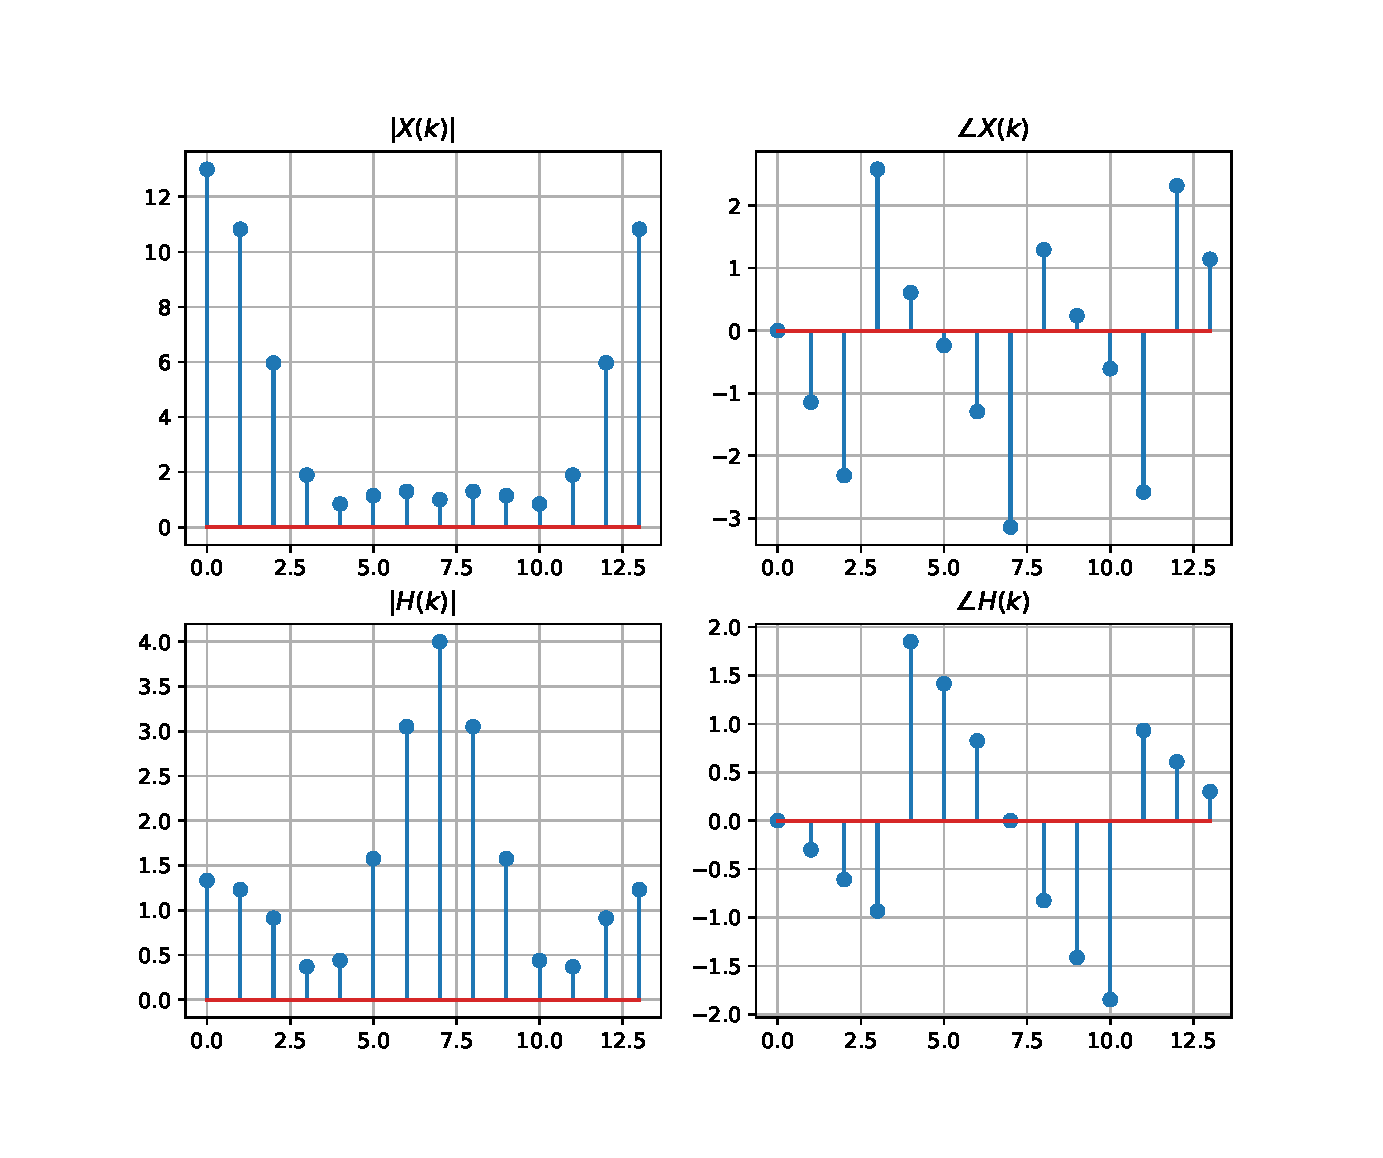
\includegraphics[width=8cm]{figs/XH_fft.eps}
\end{figure}
\subsection{Filter Output y(n)}
\end{frame} 
\begin{frame}{Filter Output Using FFT and IFFT}
\begin{itemize}
    \item $y(n)$ can be computed by doing IFFT for $Y(k)$
    \[y(n) = \frac{1}{N}\sum_{n=0}^{N-1}Y(k) e^{j 2 \pi n k / N}, \quad k=0,1, \ldots, N-1\]
\end{itemize}
\begin{figure}
    \centering
    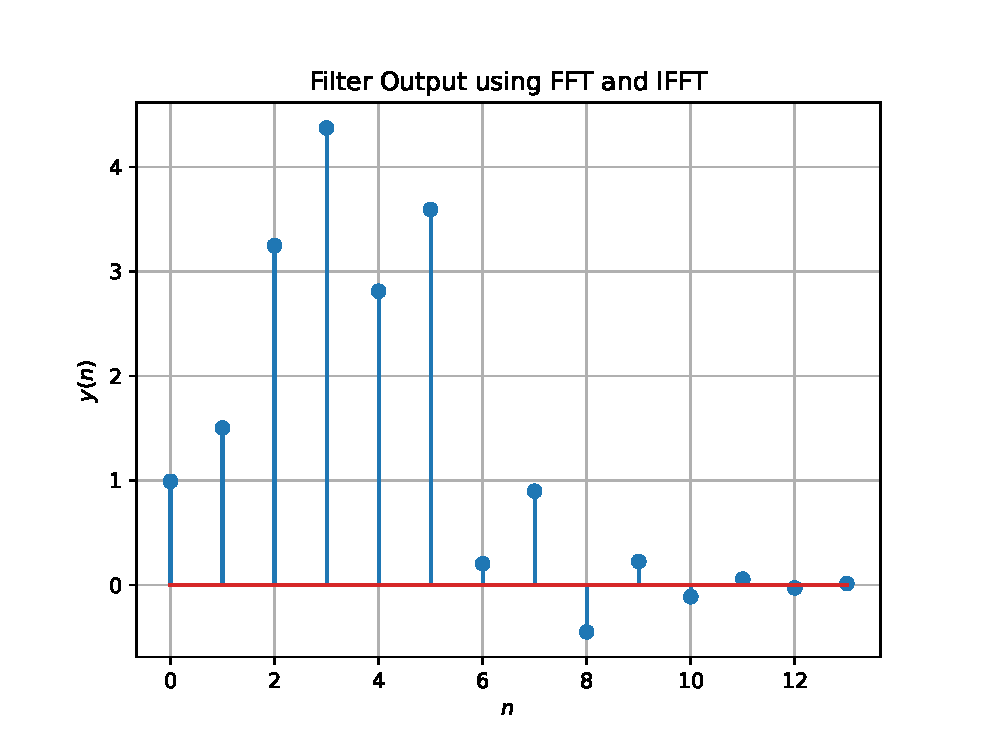
\includegraphics[width=6cm]{figs/y_n.eps}
\end{figure}
\end{frame}

\section{Matrix Equations}
\begin{frame}{expressing all the above equations as matrix equations}
\begin{itemize}
       \item FFT of signal X(n) 
   \[
        X(k) \triangleq \sum_{n=0}^{N-1} x(n) e^{-j 2 \pi k n / N}, \quad k=0,1, \ldots, N-1
    \]
    \item Let $W_{N}^{n k}=e^{-j 2 \pi k n / N}$ then this can be $\mathrm{ex}-$ pressed interms of matrices as:
    
       \[ \begin{bmatrix} X(0) \\ X(1) \\ X(2) \\ X(3) \\ X(4) \\ X(5) \end{bmatrix}
=
\begin{bmatrix}
1 & 1 & 1 & 1 & 1 & 1 \\ 1 & W_N^1& W_N^2& W_N^3 & W_N^4 & W_N^5\\1 & W_N^2 & W_N^4 & W_N^6 & W_N^8 & W_N^{10}\\1 & W_N^3 & W_N^6 & W_N^9 & W_N^{12} & W_N^{15}\\1 & W_N^4 & W_N^8 & W_N^{12} & W_N^{16} & W_N^{20}\\1 & W_N^5 & W_N^{10} & W_N^{15} & W_N^{20} &W_N^{25}
\end{bmatrix}\begin{bmatrix}
x(0) \\ x(1) \\ x(2) \\ x(3) \\ x(4) \\x(5)
\end{bmatrix}\]
\end{itemize}



\end{frame}
 \begin{frame}{Computing X(K) from Matrix Equations}
  \begin{itemize}
      \item
On solving we get,
\[\implies X(0) = 13 + 0j,\]
\[X(1) = -4 - 1.732j,\]
\[X(2) = 1 + 0j\]
\[X(3) = -1 + 0j,\]
\[X(4) = 1 + 0j,\]
\[X(5) = -4 + 1.732j\]
\item the impluse
\[
 h(n)=\frac{-1}{2}^nu(n) + \frac{-1}{2}^{n-2}u(n-2)
\]
assuming that length of h(n) is same as length of x(n) i.e.,\\ N = 6.
Similarly like x(n), solving h(n) using matrix method for each value of k we get,
  \end{itemize}  
\end{frame}

\begin{frame}{Computing H(K) from Matrix Equations}

       \[
    \begin{bmatrix} H(0) \\ H(1) \\ H(2) \\ H(3) \\ H(4) \\ H(5) \end{bmatrix}
=
\begin{bmatrix}
h(0) + h(1) + h(2) + h(3) + h(4) + h(5) \\h(0) + h(1)e^{-j\pi /3} + ... + h(5)e^{-j5\pi /3}\\h(0) + h(1)e^{-2j\pi /3} + ... + h(5)e^{-2j5\pi /3}\\h(0) + h(1)e^{-3j\pi /3} + ... + h(5)e^{-3j5\pi /3}\\
h(0) + h(1)e^{-4j\pi /3} + ... + h(5)e^{-4j5\pi /3}\\h(0) + h(1)e^{-5j\pi /3} + ... + h(5)e^{-5j5\pi /3}
\end{bmatrix}
\]  \\~\\
 On solving we get\\
H(0) = 1.28125 + 0j \;,
H(1) = 0.51625 - 0.5141875j \; ,\\
H(2) = -0.078125 + 1.1095625j \;,
H(3) = 3.84375 + 0j \;,\\
H(4) = -0.071825 - 1.1095625j \;,
H(5) = 0.515625 + 0.5141875j

\end{frame}

\begin{frame}{Computing Y(K) from Matrix Equations}
We can now compute Y(k) using below equation
   \[ Y(k) = X(k)H(k)\]
So, Y(k) is obtained element wise multiplication of X(k) and H(k)

 \[
\begin{bmatrix} 
Y(0) \\ Y(1) \\ Y(2) \\ Y(3) \\ Y(4) \\ Y(5) 
\end{bmatrix}
=
\begin{bmatrix}
16.6562+0j \\ -2.95312+1.16372j \\ -0.07812+1.10959j \\ -3.84375-9.27556j \\ -0.07812-1.10959j \\ -2.95312-1.16372j 
\end{bmatrix}\]


\end{frame}
\begin{frame}{Computinh y(n) from IFFT of Y matrix}
   
y(n) is given by IFFT of Y matrix. this y(n) can be calculated by a python code 

\[
    \begin{bmatrix} 
y(0) \\ y(1) \\ y(2) \\ y(3) \\ y(4) \\ y(5) 
\end{bmatrix}
=
\begin{bmatrix}
1.125     +0j \\ 2.28125071+0j \\ 2.6250019 -1.11022302 \times 10^{-16}j \\ 4.37499667-1.47104551\times 10^{-15}j \\ 2.6562481 +6.10622664 \times 10^{-16}j \\ 3.59375262-1.60982339 \times 10^{-15}j 
\end{bmatrix}
\]
\end{frame}
\section{Filter Design}
\begin{frame}{Filter Design Specifications}
\begin{itemize}
    \item \textbf{Tolerances:}\\
The magnitude of resonance in Pass-band is called Pass-band Tolerance and
similarly magnitude of resonance in Stop-band is called Stop-band Tolerance.\\~\\
\item \textbf{Passband:}\\
The Frequency band within which signals are transmitted by filter without
attenuation.\\~\\

\item \textbf{Stopband:}\\
The Frequency band within which signals are not transmitted by filter or with a large attenuation.\\~\\
\end{itemize}
\end{frame}
\subsection{The Bilinear Transform}
\begin{frame}{The Bilinear Transform}
    \smallskip \hspace{2ex} It is a technique in Signal Processing that is used to Continuous-Time System
Representations to Discrete-Time System Representations and vice-versa. The bilinear transform is a first-order approximation of the natural logarithm function that is an exact mapping of the z-plane to the s-plane. When the Laplace transform is performed on a discrete-time signal (with each element of the discrete-time sequence attached to a correspondingly delayed unit impulse), the result is precisely the $\mathrm{Z}$ transform of the discrete-time sequence with the substitution of $z=e^{s t}$\\~\\
\textbf{Small Proof:}

$z=e^{s T}$
$s=\frac{1}{T} \ln (z)$
$s=\frac{2}{T}\left[\frac{z-1}{z+1}+\frac{1}{3}\left(\frac{z-1}{z+1}\right)^{3}+\frac{1}{5}\left(\frac{z-1}{z+1}\right)^{5}+\frac{1}{7}\left(\frac{z-1}{z+1}\right)^{7}+\cdots\right]$
$s=\frac{2}{T} \frac{1-z^{-1}}{1+z^{-1}}$
\end{frame}
\begin{frame}{The Bilinear Transform}
$H_{d}(z)=\left.H_{a}(s)\right|_{s=\frac{2}{T} \frac{z-1}{z+1}}=H_{a}\left(\frac{2}{T} \frac{z-1}{z+1}\right)$\\~\\

$H_{d}\left(e^{j \omega_{d} T}\right)=H_{a}\left(\frac{2}{T} \frac{e^{j \omega_{d} T}-1}{e^{j \omega_{d} T+1}}\right)$\\~\\

$H_{d}\left(e^{j \omega_{d} T}\right)=H_{a}\left(\frac{2}{T} \cdot \frac{\left(e^{j \omega_{d} T / 2}-e^{-j \omega_{d} T / 2}\right)}{\left(e^{j \omega_{d} T / 2}+e^{-j \omega_{d} T / 2}\right)}\right)$\\~\\

$H_{d}\left(e^{j \omega_{d} T}\right)=H_{a}\left(j \frac{2}{T} \cdot \frac{\sin \left(\omega_{d} T / 2\right)}{\cos \left(\omega_{d} T / 2\right)}\right)$\\~\\

$H_{d}\left(e^{j \omega_{d} T}\right)=H_{a}\left(j \frac{2}{T} \cdot \tan \left(\omega_{d} T / 2\right)\right)$\\~\\

$\omega_{a}=\frac{2}{T} \tan \left(\omega_{d} \frac{T}{2}\right)$
\end{frame}
\subsection{The FIR Filter}
\begin{frame}{The FIR Filter}
The lowpass filter has a pass frequency $\omega_{l}$ and transition band $\Delta \omega$ with Stop Band Tolerance $\delta$ is
$h_{l p}(n)=\frac{\sin \left(n \omega_{l}\right)}{n \pi} w(n)$
$w(n)=\left\{\begin{array}{l}\frac{l\left[\beta N \sqrt{1-\left(\frac{n}{N}\right)^{2}}\right]}{l_{0}(\beta N)}, \quad-N \leq n \leq N, \quad \beta>0 \\ 0 \text { otherwise }\end{array}\right.$

where $w(n)$ is Kaiser Window and $I_{0}(x)$ is the modified Bessel function of the first
kind of order zero in $x$, and $N$ are the window shaping factors and they are selected
as follows\\
$ N \geq \frac{A-8}{4.57 \Delta \omega} $\\
$ A=-20 \log _{10} \delta $\\

$\beta N=\left\{\begin{array}{ll}0.1102(A-8.7) & A>50 \\ 0.5849(A-21)^{0.4}+0.07886(A-21) & 21 \leq A \leq 50 \\ 0 & A<21\end{array}\right.$
\end{frame}

\begin{frame}{The FIR Filter}
The FIR Bandpass Filter:
The centre of the passband of the desired bandpass filter was found to be $\omega_{c}=0.275 \pi$ The impulse response of the desired bandpass filter is obtained from the
impulse response of the corresponding lowpass filter as
$$
h_{b p}(n)=2 h_{l p}(n) \cos \left(n \omega_{c}\right)
$$

\begin{figure}
    \centering
    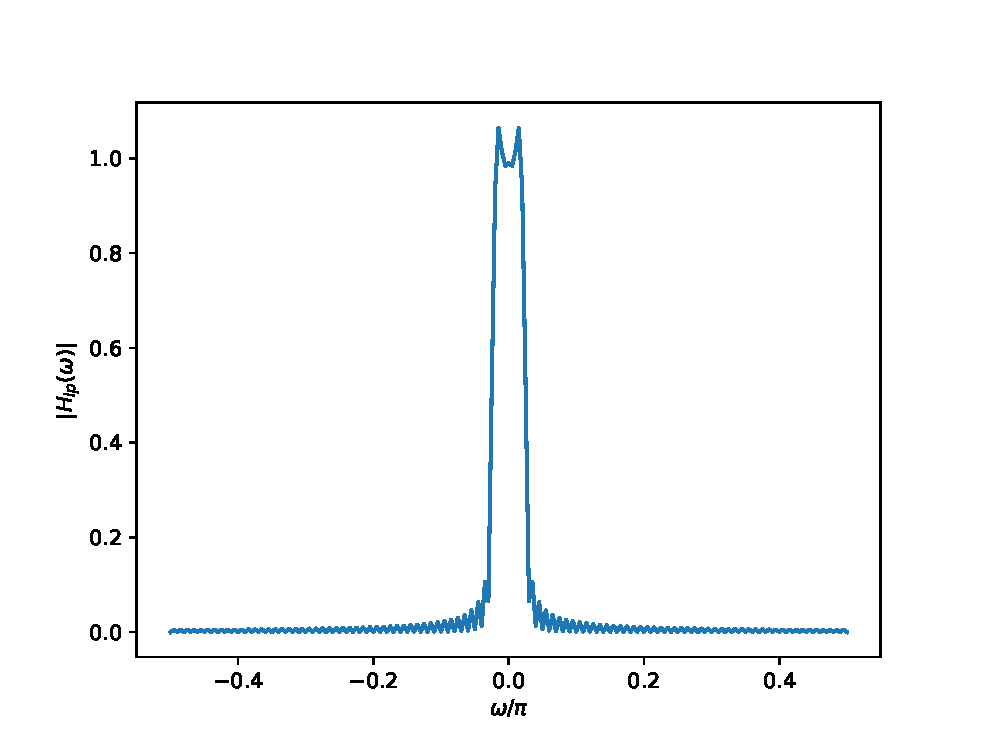
\includegraphics[width=6cm]{figs/FIR_lowpass.eps}
    \caption{FIR Low Pass Filter}
\end{figure}
\end{frame}

\begin{frame}{The FIR Filter}

\begin{figure}
    \centering
    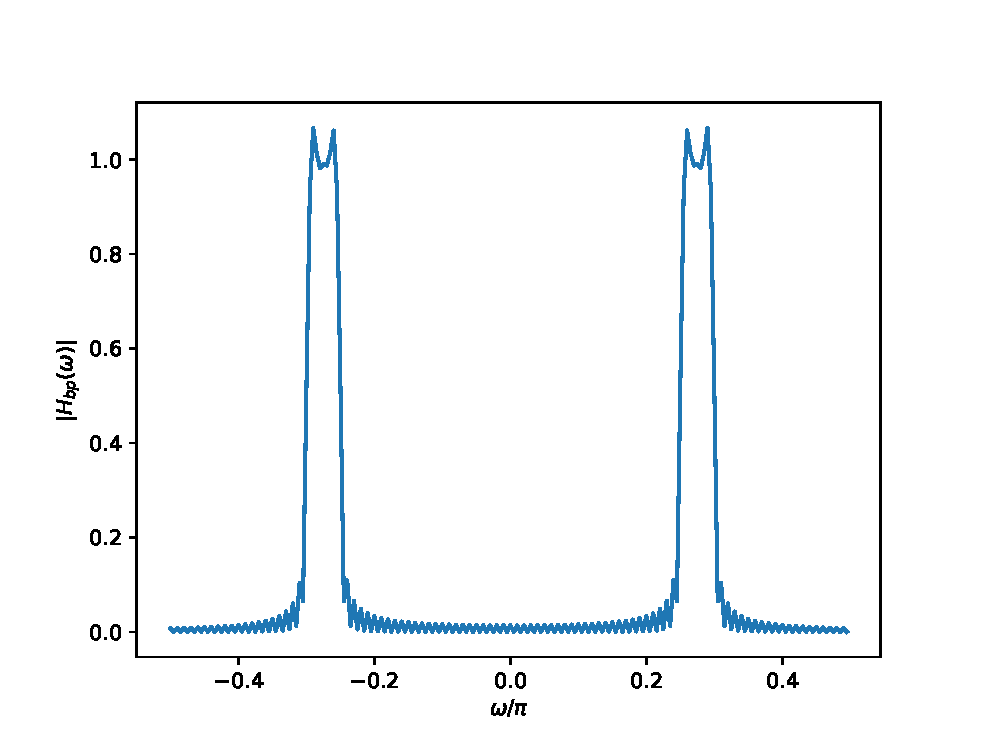
\includegraphics[width=6cm]{figs/FIR_bandpass.eps}
    \caption{FIR Low Pass Filter}
\end{figure}

\noindent
{\definecolor{arsenic}{rgb}{0.23, 0.27, 0.29} \rule{\linewidth}{0.5mm} }
\definecolor{arsenic}{rgb}{0.23, 0.27, 0.29}
\Huge{\centerline{Thank You}}
\noindent
{\definecolor{arsenic}{rgb}{0.23, 0.27, 0.29} \rule{\linewidth}{0.5mm} }
\end{frame}


\end{document}
